\section{Video Player}
\subsection{Ziel}
Um manipulationen im Cockpit zu in unserem Programm zu empfangen zu zu verarbeiten, wird in einem ersten Schritt ein Video-Player realisiert der auf Eingaben des Probanden reagiert. Dies gibt ebenfalls einen ersten Eindruck von einem Fahrverhalten auf dem Simulator. Bei einem Video ist nur die Geschwindigkeit und noch keine Richtung und weiters relevant. Somit wird mit dem Video-Player die Ausgabe sehr reduziert. Ziel im Video-Player ist eine korrekte Übertragung der Eingaben im Cockpit über LabVIEW in das Programm. Das Programm soll die Parameter richtig interpretieren und entsprechende Aktionen veranlassen. Ein weiteres Ziel ist ein korrekte Rückgabe verschiedener Parameter an LabVIEW die von diesem in eine LogDatei geschrieben werden. 
\subsection{Systembeschreibung}

% Bild für Systembeschreibung des Video Players
\begin{figure}[H]
\centering 
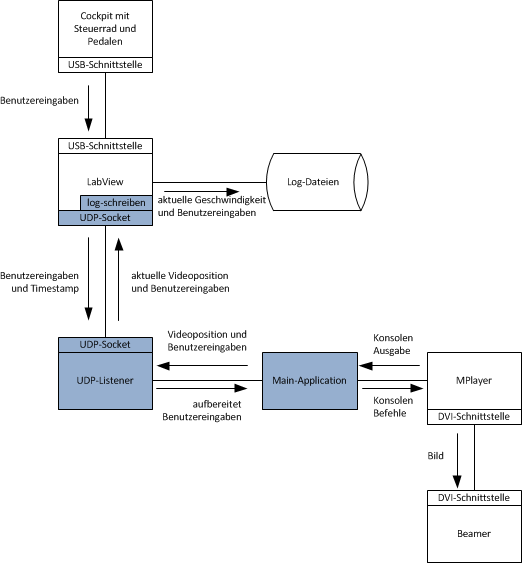
\includegraphics{src/Systembeschreibung_VideoPlayer.png}
\caption{Systembeschreibung Video-Player} % Titel der Grafik
\label{Systembeschreibung Video-Player} % Labelname
\end{figure}
Um einzelne Komponenten des Video-Player wiederverwenden zu können, wird das System möglichst gleich wie das des Fahrsimulators aufgebaut. Dieser Aufbau wird anhand der Abbildung \ref{Systembeschreibung Video-Player} illustriert.  Die blau markierten Komponenten werden im Rahmen des Video-Players entwickelt. Alle überigen sind bereits vorbestehend oder werden installiert und verwendet. 
Die LabVIEW-Komponente in der Abbildung \ref{Systembeschreibung Video-Player} liest bereits die Eingaben die der Proband im Cockpit mach ein. Dieses muss nun so erweitert werden, dass diese über einen UDP-Socket an das Programm übertragen werden. Zusätzlich muss im LabVIEW ein UDP-Port eingerichtet werden, der verwendet werden kann, um UDP-Packete zu empfangen. Dieser wird benötigt um Daten die von unserem Programm gesendet werden in ein Log-File zu schreiben.
Die Parameter werden vom vom UDP-Listener gespeichert und vom Hauptprogramm abgefragt. Aufgrund der Parameter wird dann die Geschwindigkeit des Videos manipuliert. Für das Abspielen des Videos wird der mPlayer verwendet. Die Befehle für den mPlayer können von unserem Programm über die Komandozeile abgesetzt werden. Ausgaben vom mPlayer  werden ebenfalls über die Komandozeile den Standartausgang der Konsole übergeben. 

\subsection{Realisierung}
In einem bestehendem LabVIEW-Programm werden bereits alle Eingaben, die im Cockpit gemacht werden können, eingelesen. Nun muss dieses Programm nur noch mit einem UDP-Port erweitert werden, damit es die Parameter, die unser Video-Player benötigt, senden kann. Diese Daten sind im Video-Player vor allem die betätigung von Gas- und Bremspedal. Diese beiden Pedalen werden in einem Koordinatensystem auf der y-Achse abgebildet. Die positive y-Richtung verifiziert das Gas und die negative y-Richtung das Bremspedal. Die intensität beider Pedalen wird durch 32767 bzw. 32768 ganzzahlige Werte identifiziert. 

\begin{figure}[H]
\centering 
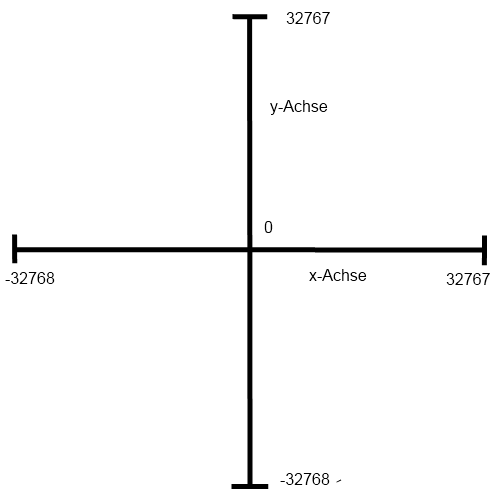
\includegraphics{src/koordinatensystem.png}
\caption{Koordinatensystem} % Titel der Grafik
\label{Koordinatensystem} % Labelname
\end{figure}
Daten x und y verifiziert